\documentclass[portrait,final,a1paper,fontscale=0.3]{baposter}

\usepackage{calc}
\usepackage{graphicx}
\usepackage{amsmath}
\usepackage{amssymb}
\usepackage{relsize}
\usepackage{multirow}
\usepackage{rotating}
\usepackage{bm}
\usepackage{url}

\usepackage{graphicx}
\usepackage{multicol}
\usepackage{amsthm}
\usepackage{amssymb}
\usepackage{mathtools}
\DeclarePairedDelimiter\abs{\lvert}{\rvert}
\DeclarePairedDelimiter\norm{\lVert}{\rVert}
\DeclarePairedDelimiter\inner{\langle}{\rangle}
\def\P{\mathcal{P}}
\DeclareMathOperator*{\argmin}{argmin}
\theoremstyle{definition}
\newtheorem{definition}{Definition}
\newtheorem{proposition}{Proposition}
\newtheorem{example}{Example}
\newtheorem{lemma}{Lemma}
\newtheorem{corollary}{Corollary}
\newtheorem{theorem}{Theorem}
\usepackage{algorithm}
\usepackage{algorithmic}
\makeatletter
\newcommand{\algorithmicfunction}{\textbf{function}}
\newcommand{\algorithmicendfunction}{\algorithmicend\ \algorithmicfunction}
\newenvironment{ALC@func}{\begin{ALC@g}}{\end{ALC@g}}
\newcommand{\FUNCTION}[2][default]{\ALC@it\algorithmicfunction\ #2\ %
\textbf{:}%
\ALC@com{#1}\begin{ALC@func}}
\ifthenelse{\boolean{ALC@noend}}{
    \newcommand{\ENDFUNCTION}{\end{ALC@func}}
  }{
    \newcommand{\ENDFUNCTION}{\end{ALC@func}\ALC@it\algorithmicendfunction}
  }
\makeatother

\usepackage{palatino}

\newcommand{\captionfont}{\footnotesize}


\setlength{\columnsep}{1.5em}
\setlength{\columnseprule}{0mm}

\newcommand{\compresslist}{%
\setlength{\itemsep}{1pt}%
\setlength{\parskip}{0pt}%
\setlength{\parsep}{0pt}%
}


\begin{document}


\definecolor{stevensred}{HTML}{82318E}
\definecolor{stevensgray}{rgb}{0.60392, 0.596, 0.60392}

\begin{poster}%
  {
  grid=false,
  colspacing=1em,
  bgColorOne=white,
  bgColorTwo=white,
  borderColor=stevensgray,
  headerColorOne=stevensred,
  headerColorTwo=stevensred,
  headerFontColor=white,
  boxColorOne=white,
  boxColorTwo=stevensgray,
  textborder=rectangle,
  eyecatcher=true,
  headerborder=closed,
  headerheight=0.13\textheight,
  headershape=rectangle,
  headershade=shadelr,
  headerfont=\Large\bf\textsc, %Sans Serif
  textfont={\setlength{\parindent}{1.5em}},
  boxshade=plain,
  background=plain,
  linewidth=2pt
  }
  {
  		
\includegraphics[height=9.0em]{thu.jpg}
  } % Empty space, replace with image if desired
  {\bf \textsc{ Info-Detection: An Information-Theoretic Approach to Detect Outlier } }
  {\textsc{  Feng Zhao, Fei Ma, Yang Li, Shao-Lun Huang and Lin Zhang \\ Tsinghua-Berkeley Shenzhen Institute, Tsinghua University}}
  {% The makebox allows the title to flow into the logo, this is a hack because of the L shaped logo.
  }

    \newcommand{\colouredcircle}{%
      \tikz{\useasboundingbox (-0.2em,-0.32em) rectangle(0.2em,0.32em); \draw[draw=black,fill=lightblue,line width=0.03em] (0,0) circle(0.18em);}}

  \headerbox{Introduction}{name=problem,column=0,row=0}{

Outlier detection is one of major task in unsupervised learning. We propose a cluster analysis based method called Info-Detection. It can determine the number of outliers automatically. To implement Info-Detection, we use some graph theory techniques and make it usable on small dataset.

}

  \headerbox{References}{name=references,column=0,above=bottom}{
    \smaller
    \bibliographystyle{ieee}
    \renewcommand{\section}[2]{\vskip 0.05em}
      \begin{thebibliography}{1}\itemsep=-0.01em
      \setlength{\baselineskip}{0.4em}
      
\bibitem{sparsekernel} C.~Chan, A.~Al-Bashabsheh, Q.~Zhou, T.~Kaced, and T.~Liu.
\newblock Info-clustering: A mathematical theory for data clustering.
\newblock {\em IEEE Transactions on Molecular, Biological and Multi-Scale
  Communications}, 2(1):64--91, 2016.
  
\bibitem{RN4}
Vladimir Kolmogorov.
\newblock A faster algorithm for computing the principal sequence of partitions
  of a graph.
\newblock {\em Algorithmica}, 56(4):394--412, 2010.

\bibitem{RN7}
Kiyohito Nagano, Yoshinobu Kawahara, and Satoru Iwata.
\newblock Minimum average cost clustering.
\newblock {\em Advances in Neural Information Processing
  Systems 23}, pages 1759--1767. Curran Associates, Inc., 2010.

      \end{thebibliography}
   \vspace{0.05em}
  }

  \headerbox{Info-clustering}{name=method,column=0,below=problem, above=references}{
Info-Detection derives from info-clustering.
Info-clustering is an information theoretic clustering method and can produce hierachical tree for the random variables to be clustered. 
Consider a graph $G(V, E)$ 
}

\headerbox{Algorithm}{name=results,column=1,span=2,row=0}{

\begin{multicols}{2}

The clustering result can be achieved by solving the principal sequence of partition for the input graph.
\begin{align}\label{eq:hL}
	h_{\P}(\lambda) &=  f[\P] - \abs{\P} \lambda  \\
	h(\lambda) &= \min_{\P \in \Pi'(V)} h_{\P}(\lambda)
\end{align}
Solving the following problem sequentially for $t=1,\dots,\abs{V}$ (\textsf{pdt}).
\begin{align}
	\tilde{h}_{\lambda}(T) &= f(T) - \lambda - y^{\lambda}(T)\\
	\tilde{h}(\lambda) & = \min_{t \in T \subseteq V} \tilde{h}_{\lambda}(T) \label{eq:pmq}
\end{align}
\begin{theorem}[Principal Sequence]
	\begin{align}\notag
		T^{\lambda} & =\begin{cases}
			T_0 & \lambda < \lambda_1 \\
			T_i & \lambda_i \leq \lambda < \lambda_{i+1}\\
			T_k & \lambda \geq \lambda_{k}
		\end{cases} \\
		T_k & \subsetneq  \dots \subsetneq T_1 \subsetneq T_0 \label{eq:Alambda}				
	\end{align}
\end{theorem}
{
		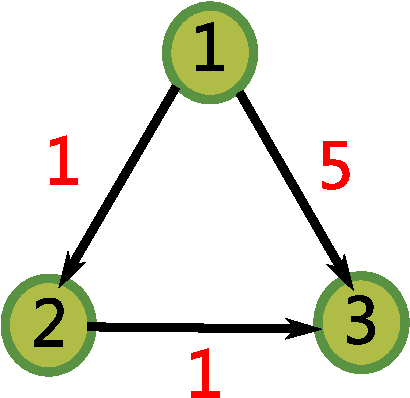
\includegraphics[width=0.27\linewidth]{img/example_directed.pdf}~
		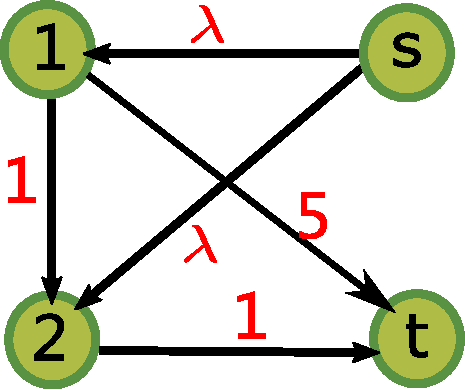
\includegraphics[width=0.3\linewidth]{img/example_st.pdf}~
		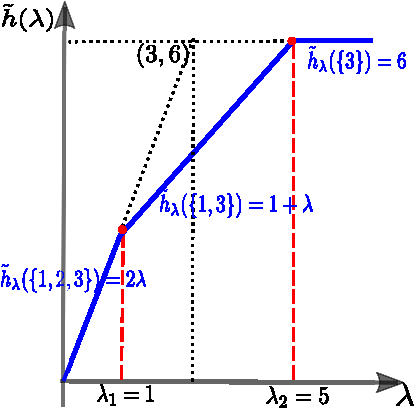
\includegraphics[width=0.27\linewidth]{img/example_pst_single.pdf}
}

To compute $\tilde{h}(\lambda)$, we combine Algorithm and \textsf{pmf}.

{

}
\begin{multicols}{2}		
Converting $G$ to $\widetilde{G}$ by adding $s$ and modifying weights.
Starting from a given flow map when computing $P'$.

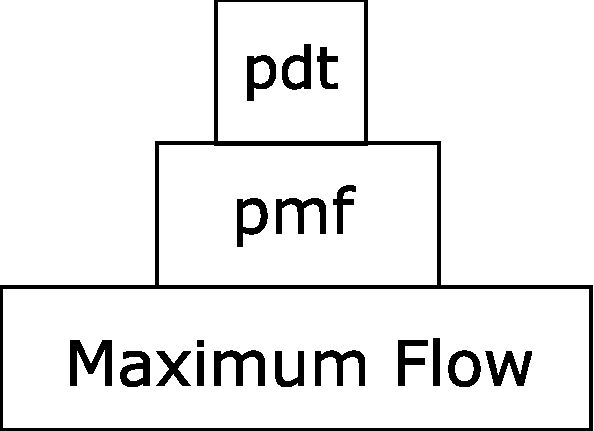
\includegraphics[width=0.65\linewidth]{img/pdt.pdf}
\end{multicols}
\end{multicols}

}

\headerbox{How to choose graph weight}{name=example,below=results,column=1,span=2}{
	\begin{multicols}{2}
The clustering tree has no stem nodes if and only if
\begin{equation}
	\frac{f[\P]}{\abs{\P}-1} \geq \frac{\sum_{(i,j) \in E} w_{ij}}{\abs{V}-1}				
\end{equation}
holds for any partition $\abs{\P} > 1$.

If $w_{ij} + w_{jk} \geq w_{ki}$ for any different triple $i, j, k \in V$, then the clustering tree has no stem nodes.

Suppose $S_1, S_2 $ are complete graph with size $n$ equal weight $w_{ij}=n$. There are $m$ edges between the two graphs and all inter-connection edges have equal weight 1. Then for $V=S_1\cup S_2$, we have
	\end{multicols}
}

  \headerbox{Experimental Results}{name=experiment,column=1, span=2,below=example, above=bottom}{
\begin{multicols}{2}
We tested our method "graph-based info-clustering" to cluster multi-dimensional vectors. We prepare three groups of data.

\textbf{1)} Four Gaussian blobs 

\textbf{2)} Three concentric circles

\textbf{3)} UCI glass dataset with 214 samples, 6 classes

clustering result of Gaussian and Circle dataset is shown on above figure.
\\

In some parameter combination, the hierarchical tree obtained by graph-based info-clustering is the same as that of the ground truth.\\

{
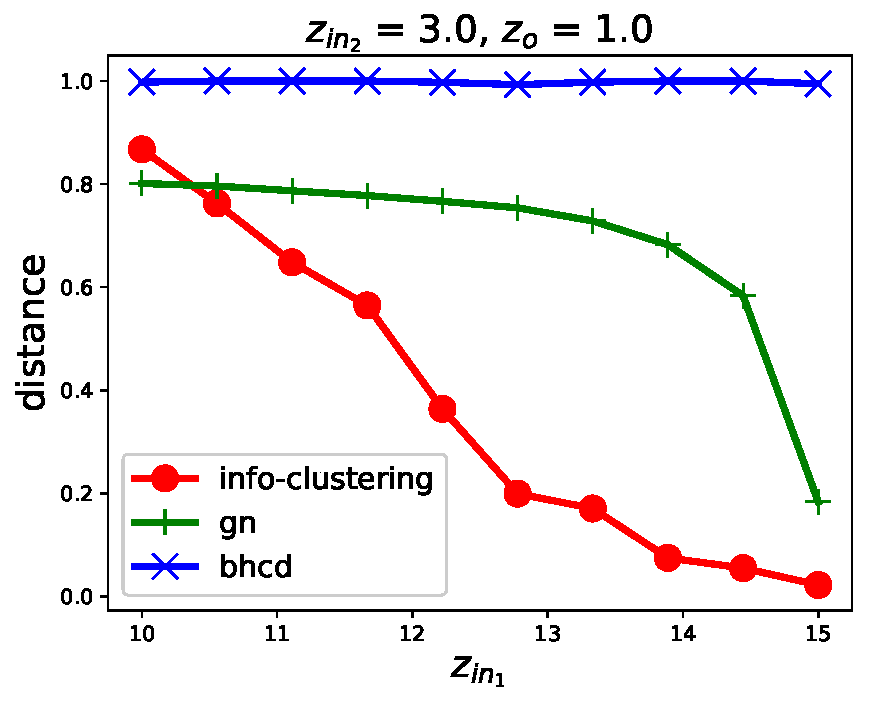
\includegraphics[width=0.46\linewidth]{img/z_in_1.pdf}
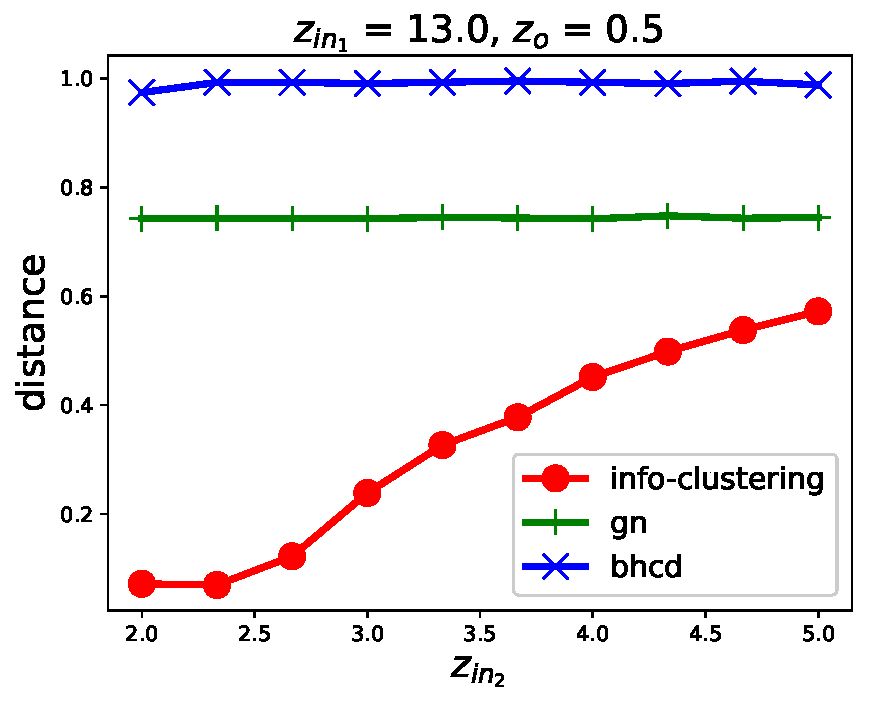
\includegraphics[width=0.46\linewidth]{img/z_in_2.pdf}
}

\end{multicols}

}


\end{poster}

\end{document}

